% kassett.tex -- kassetten i ABC80 och ABC 800-serien, med figurer.
% Byggs med bygg.sh (tectonic) till kassett.pdf. Underlaget är
% ../FORMAT.md och ../HARDVARA.md; (?) betyder att uppgiften inte är belagd.
\documentclass[10pt]{article}
\usepackage[paperwidth=190mm,paperheight=270mm,left=21mm,right=21mm,
  top=20mm,bottom=22mm]{geometry}
\usepackage{fontspec}
\usepackage[swedish]{babel}
\setmainfont{texgyrepagella}[Extension=.otf,UprightFont=*-regular,
  BoldFont=*-bold,ItalicFont=*-italic,BoldItalicFont=*-bolditalic]
\setmonofont{Inconsolatazi4-Regular.otf}[BoldFont=Inconsolatazi4-Bold.otf,
  Scale=0.92]
\usepackage{xcolor}
\usepackage{array,booktabs}
\usepackage{tikz}
\usetikzlibrary{arrows.meta,positioning,calc,decorations.pathreplacing,
  shapes.geometric,fit}
\usepackage{caption}
\usepackage{float}
\floatplacement{figure}{H}
\captionsetup{font=small,labelfont=bf,labelsep=period}
\usepackage[colorlinks,linkcolor=black!70!blue,urlcolor=black!70!blue]{hyperref}
\hypersetup{pdftitle={Kassetten i ABC-datorerna}}
\setlength{\parindent}{0pt}
\setlength{\parskip}{0.6\baselineskip}
\definecolor{fut}{HTML}{3B6EA8}   % det som skrivs
\definecolor{fin}{HTML}{B5543A}   % det som läses
\definecolor{gra}{gray}{0.88}
\definecolor{mork}{gray}{0.35}
\newcommand\kw[1]{\texttt{#1}}
\newcommand\adr[1]{\texttt{\$#1}}
\newcommand\namn[1]{\textsc{\MakeLowercase{#1}}}
\tikzset{
  sig/.style={line width=1pt},
  cell/.style={draw=mork,densely dotted,line width=0.4pt},
  ruta/.style={draw,rounded corners=2pt,align=center,inner sep=4pt,
    font=\small},
  fil/.style={draw,fill=gra,align=center,inner sep=4pt,font=\small},
  pil/.style={-{Stealth[length=2.2mm]},line width=0.6pt},
  bit/.style={font=\small\ttfamily},
}

\begin{document}

\begin{center}
{\LARGE\bfseries Kassetten i ABC-datorerna\par}
\medskip
{\large Signalen, blocken, filerna och verktygen\par}
\medskip
{\small ABC80, ABC 800 C/M, ABC 802 och ABC 806\par}
\end{center}

\bigskip

ABC80 och datorerna i ABC 800-serien sparar program och data på en vanlig
ljudkassett. Här beskrivs hur: vilken signal som står på bandet, hur den
blir block och filer, hur ROM:en skriver och läser den, och hur
verktygen i \kw{kassett/} flyttar filerna mellan bandet och dagens
datorer. Uppgifterna kommer ur ROM:erna, ur schemat för ABC 800 och ur
Markesjö 1978. Det som inte är belagt är märkt med (?).

\begin{figure}[H]
\centering
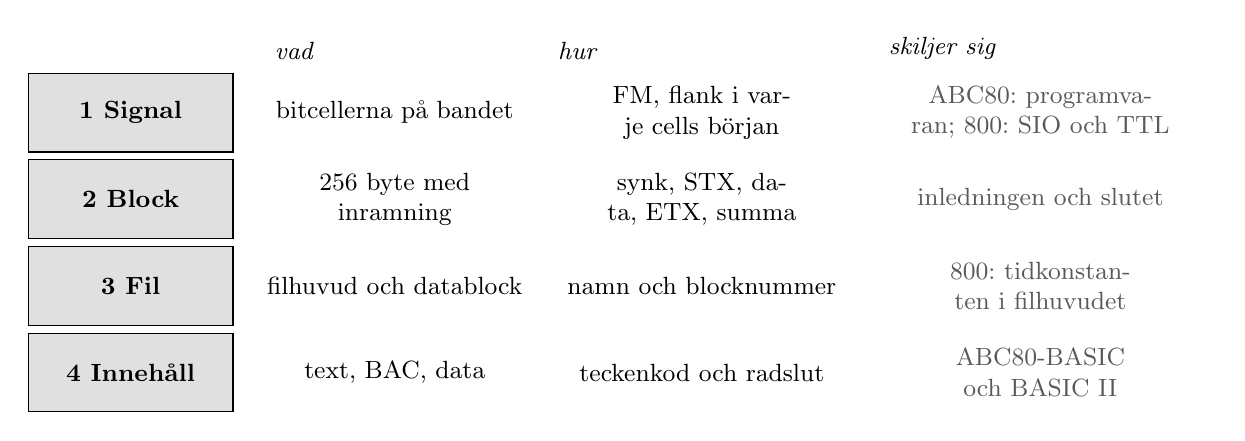
\begin{tikzpicture}[node distance=0mm]
\foreach \n/\t/\d/\s [count=\i] in {
  {1 Signal}/{bitcellerna på bandet}/{FM, flank i varje cells början}/{ABC80: programvaran; 800: SIO och TTL},
  {2 Block}/{256 byte med inramning}/{synk, STX, data, ETX, summa}/{inledningen och slutet},
  {3 Fil}/{filhuvud och datablock}/{namn och blocknummer}/{800: tidkonstanten i filhuvudet},
  {4 Innehåll}/{text, BAC, data}/{teckenkod och radslut}/{ABC80-BASIC och BASIC II}}{
  \node[fil,minimum width=26mm,minimum height=10mm,anchor=north west]
    (l\i) at (0,-\i*11mm) {\bfseries\n};
  \node[ruta,draw=none,minimum height=10mm,text width=34mm,anchor=west]
    at ($(l\i.east)+(2mm,0)$) {\t};
  \node[ruta,draw=none,minimum height=10mm,text width=40mm,anchor=west]
    at ($(l\i.east)+(38mm,0)$) {\d};
  \node[ruta,draw=none,minimum height=10mm,text width=42mm,anchor=west,
    text=mork] at ($(l\i.east)+(80mm,0)$) {\s};
}
\node[font=\small\itshape,anchor=south west] at ($(l1.north east)+(4mm,0.5mm)$) {vad};
\node[font=\small\itshape,anchor=south west] at ($(l1.north east)+(40mm,0.5mm)$) {hur};
\node[font=\small\itshape,anchor=south west] at ($(l1.north east)+(82mm,0.5mm)$) {skiljer sig};
\end{tikzpicture}
\caption{En fil på bandet i fyra lager. Avsnitten nedan går uppifrån och ned.}
\end{figure}

\section{Signalen}

Signalen är FM (bifas): den vänds i början av varje bitcell, och en etta
vänds en gång till mitt i cellen. Det är alltså antalet flanker per cell,
inte nivån, som bär biten, och därför spelar det ingen roll om
bandspelaren vänder signalen. Den minst signifikanta biten skrivs först.

\begin{figure}[H]
\centering
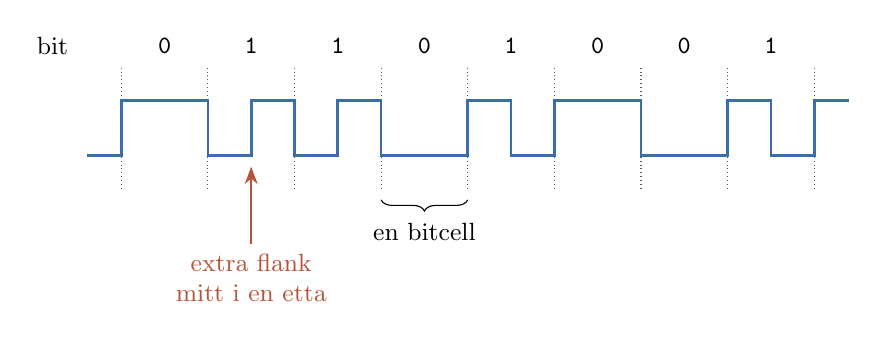
\begin{tikzpicture}[x=11mm,y=7mm]
% bitarna 0 1 1 0 1 0 0 1
\def\bitar{0,1,1,0,1,0,0,1}
\foreach \b [count=\i from 0] in \bitar {
  \draw[cell] (\i,-0.6) -- (\i,1.6);
  \node[bit] at (\i+0.5,2.0) {\b};
}
\draw[cell] (8,-0.6) -- (8,1.6);
% vågen: start låg
\draw[sig,fut]
  (-0.4,0) -- (0,0) -- (0,1) -- (1,1) -- (1,0) -- (1.5,0) -- (1.5,1)
  -- (2,1) -- (2,0) -- (2.5,0) -- (2.5,1) -- (3,1) -- (3,0) -- (4,0)
  -- (4,1) -- (4.5,1) -- (4.5,0) -- (5,0) -- (5,1) -- (6,1) -- (6,0)
  -- (7,0) -- (7,1) -- (7.5,1) -- (7.5,0) -- (8,0) -- (8,1) -- (8.4,1);
\draw[decorate,decoration={brace,mirror,amplitude=4pt}]
  (3,-0.8) -- (4,-0.8) node[midway,below=5pt,font=\small] {en bitcell};
\draw[pil,fin] (1.5,-1.6) node[below,font=\small,align=center]
  {extra flank\\mitt i en etta} -- (1.5,-0.2);
\node[font=\small,anchor=east] at (-0.5,2.0) {bit};
\end{tikzpicture}
\caption{Bitarna 0 1 1 0 1 0 0 1 i FM. De prickade linjerna är cellgränserna,
och där vänds signalen alltid. En etta har en flank till i mitten.}
\end{figure}

Bitcellens längd beror på maskinen. I ABC80 räknar programmet själv ut
tiden mellan flankerna i T-cykler (klockcykler); i ABC 800-serien ger
räknaren CTC dubbla bittakten, och tidkonstanten \emph{tk} bestämmer den.

\begin{center}
\small
\begin{tabular}{@{}llrrr@{}}
\toprule
Maskin & Bitcell & Klocka & Tid & Bit/s \\
\midrule
ABC80, nolla & 3993 T & 2,9952 MHz & 1,333 ms & 750 \\
ABC80, etta & 4065 T & 2,9952 MHz & 1,357 ms & 737 \\
ABC 800, tk 129 & $32 \times 129$ T & 3 MHz & 1,376 ms & 727 \\
ABC 800, tk 40 & $32 \times 40$ T & 3 MHz & 0,427 ms & 2\,344 \\
\bottomrule
\end{tabular}
\end{center}

Luxor anger 700 respektive 700 och 2\,400 baud. I ABC80 är en etta lite
längre än en nolla, eftersom ROM:en gör två anrop i stället för ett (i
version 9913 är den 8 T kortare). I ABC 800-serien är alla celler lika
långa.

\section{Hur ABC80 skriver}

ABC80 har ingen krets för kassetten utöver tre bitar i PIO:ns port B,
\adr{3A}: bit 5 drar motorreläet, bit 6 är skrivsignalen och bit 7 den
lästa signalen. Allt annat gör ROM:en. Rutinen \namn{CASWBI} skriver biten
i CY, och \namn{CASHLF} väntar och vänder signalen.

\begin{figure}[H]
\centering
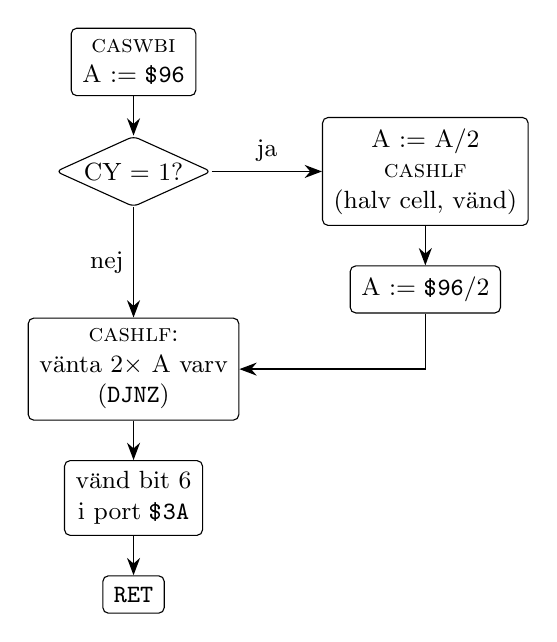
\begin{tikzpicture}[node distance=5mm and 8mm]
\node[ruta] (a) {\namn{CASWBI}\\A := \adr{96}};
\node[ruta,shape=diamond,aspect=2.2,inner sep=1pt,below=of a] (b) {CY = 1?};
\node[ruta,right=14mm of b] (c) {A := A/2\\\namn{CASHLF}\\(halv cell, vänd)};
\node[ruta,below=of c] (d) {A := \adr{96}/2};
\node[ruta,below=14mm of b] (e) {\namn{CASHLF}:\\vänta $2 \times$ A varv\\(\kw{DJNZ})};
\node[ruta,below=of e] (f) {vänd bit 6\\i port \adr{3A}};
\node[ruta,below=of f] (g) {\kw{RET}};
\draw[pil] (a) -- (b);
\draw[pil] (b) -- node[above,font=\small] {ja} (c);
\draw[pil] (c) -- (d);
\draw[pil] (d) |- (e);
\draw[pil] (b) -- node[left,font=\small] {nej} (e);
\draw[pil] (e) -- (f);
\draw[pil] (f) -- (g);
\end{tikzpicture}
\caption{En bit från ABC80. En nolla är ett varv i \namn{CASHLF} med
\adr{96}: en hel cell och sedan en flank. En etta är två varv med hälften,
alltså två flanker. \namn{CASWBY} skriver en byte bit för bit med början i
bit 0.}
\end{figure}

\section{Hur ABC80 läser}

Läsningen sker med avbrott. PIO B ger ett avbrott på flanken i början av
varje cell, och rutinen \namn{CASINT} tittar sedan efter om det har kommit
en flank till. Bit 6, som skriver vid skrivning, styr vid läsning en
låskrets som fångar flankerna (Markesjö 1978, s.~164--167).

\begin{figure}[H]
\centering
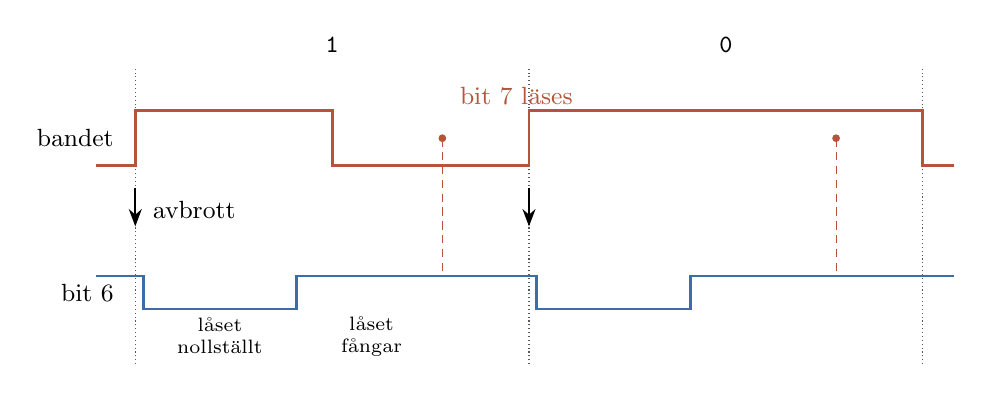
\begin{tikzpicture}[x=50mm,y=7mm]
\foreach \x in {0,1,2} \draw[cell] (\x,-3.6) -- (\x,1.8);
\node[bit] at (0.5,2.2) {1};
\node[bit] at (1.5,2.2) {0};
\node[font=\small,anchor=east] at (-0.03,0.5) {bandet};
\draw[sig,fin] (-0.1,0) -- (0,0) -- (0,1) -- (0.5,1) -- (0.5,0) -- (1,0)
  -- (1,1) -- (2,1) -- (2,0) -- (2.08,0);
% avbrotten
\foreach \x in {0,1} \draw[pil] (\x,-0.4) -- (\x,-1.1);
\node[font=\small,anchor=west] at (0.02,-0.8) {avbrott};
% bit 6
\node[font=\small,anchor=east] at (-0.03,-2.3) {bit 6};
\draw[sig,fut] (-0.1,-2) -- (0.02,-2) -- (0.02,-2.6) -- (0.41,-2.6) --
  (0.41,-2) -- (1.02,-2) -- (1.02,-2.6) -- (1.41,-2.6) -- (1.41,-2) -- (2.08,-2);
\node[font=\scriptsize,align=center] at (0.215,-3.1) {låset\\nollställt};
\node[font=\scriptsize,align=center] at (0.6,-3.1) {låset\\fångar};
% läsningen
\foreach \x in {0.78,1.78} {
  \fill[fin] (\x,0.5) circle (1.4pt);
  \draw[densely dashed,fin] (\x,0.5) -- (\x,-2);
}
\node[font=\small,text=fin,anchor=west] at (0.80,1.25) {bit 7 läses};
\end{tikzpicture}
\caption{\namn{CASINT}, steg för steg. (1) Avbrottet kommer på flanken i
cellens början. (2) Bit 6 sätts till 0, och låskretsen hålls nollställd
\adr{78} varv i \kw{DJNZ}, ungefär 0,5 ms. (3) Bit 6 sätts till 1, och
låset kan fånga en flank. (4) Efter lika lång tid till, ungefär 3/4 cell
från början, läses bit 7. Har en flank kommit i mitten av cellen är biten 1
(CY är den inverterade bit 7). Att låset fungerar just så är en tolkning
(?).}
\end{figure}

Bitarna samlas till block av en korutin: \namn{RCVBLK} är skriven som ett
vanligt program, men \namn{RCVBIT} och \namn{RCVBYT} sparar var den står och
avslutar avbrottet. När nästa bit eller byte är klar hoppar \namn{CASINT}
tillbaka dit.

\begin{figure}[H]
\centering
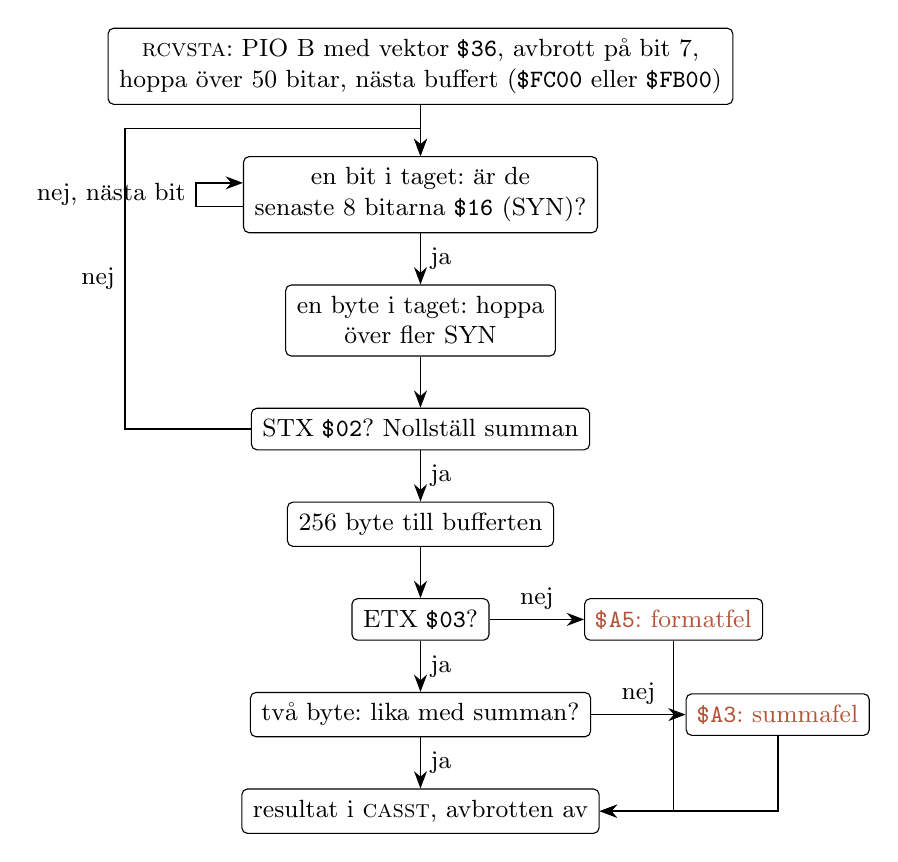
\begin{tikzpicture}[node distance=6.5mm and 8mm]
\node[ruta] (s) {\namn{RCVSTA}: PIO B med vektor \adr{36}, avbrott på bit 7,\\
  hoppa över 50 bitar, nästa buffert (\adr{FC00} eller \adr{FB00})};
\node[ruta,below=of s] (a) {en bit i taget: är de\\senaste 8 bitarna \adr{16} (SYN)?};
\node[ruta,below=of a] (b) {en byte i taget: hoppa\\över fler SYN};
\node[ruta,below=of b] (c) {STX \adr{02}? Nollställ summan};
\node[ruta,below=of c] (d) {256 byte till bufferten};
\node[ruta,below=of d] (e) {ETX \adr{03}?};
\node[ruta,below=of e] (f) {två byte: lika med summan?};
\node[ruta,below=of f] (g) {resultat i \namn{CASST}, avbrotten av};
\node[ruta,right=12mm of e,text=fin] (fe) {\adr{A5}: formatfel};
\node[ruta,right=12mm of f,text=fin] (fs) {\adr{A3}: summafel};
\draw[pil] (s) -- (a); \draw[pil] (a) -- node[right,font=\small] {ja} (b);
\draw[pil] (b) -- (c); \draw[pil] (c) -- node[right,font=\small] {ja} (d);
\draw[pil] (d) -- (e); \draw[pil] (e) -- node[right,font=\small] {ja} (f);
\draw[pil] (f) -- node[right,font=\small] {ja} (g);
\draw[pil] (e) -- node[above,font=\small] {nej} (fe);
\draw[pil] (f) -- node[above,font=\small] {nej} (fs);
\draw[pil] (fe) |- (g); \draw[pil] (fs) |- (g);
\draw[pil] ([yshift=-1.5mm]a.west) -- ++(-6mm,0) |- node[pos=0.25,left,font=\small] {nej, nästa bit} ([yshift=1.5mm]a.west);
\draw[pil] (c.west) -- ++(-16mm,0) |- node[pos=0.25,left,font=\small] {nej} ([yshift=3.5mm]a.north) -- ([yshift=0mm]a.north);
\end{tikzpicture}
\caption{\namn{RCVBLK}, korutinen som tar emot ett block. Varje pil nedåt
i den vänstra spalten väntar på en eller åtta nya avbrott. Programmet
(\namn{CASRBL}) ger fel 42 om blocket inte är klart inom ungefär 8,5 s.}
\end{figure}

\section{Blocket och summan}

Ett block har 256 byte, inramade av en inledning med nollbitar, synk och
STX före och ETX och en summa efter. De två maskinerna ramar in nästan
lika.

\begin{figure}[H]
\centering
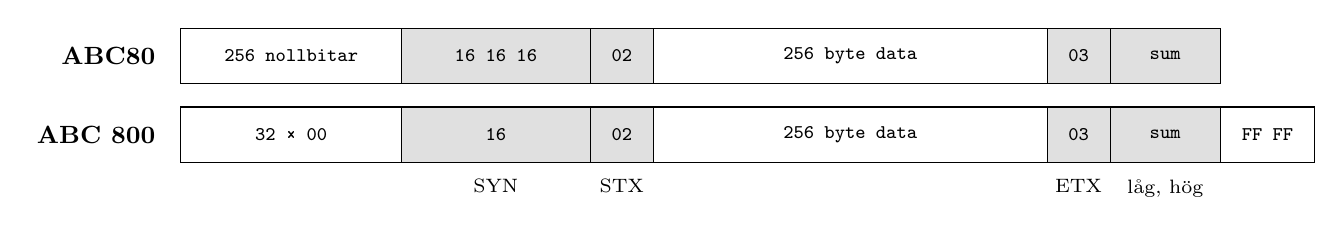
\begin{tikzpicture}[x=1mm,y=1mm]
\def\rad#1#2{\node[font=\small\bfseries,anchor=east] at (-2,#1+3.5) {#2};}
\newcommand\del[5]{% y, x, bredd, text, fyllning
  \draw[fill=#5] (#2,#1) rectangle ++(#3,7);
  \node[font=\scriptsize\ttfamily] at (#2+#3/2,#1+3.5) {#4};}
\rad{10}{ABC80}
\del{10}{0}{28}{256 nollbitar}{white}
\del{10}{28}{24}{16 16 16}{gra}
\del{10}{52}{8}{02}{gra}
\del{10}{60}{50}{256 byte data}{white}
\del{10}{110}{8}{03}{gra}
\del{10}{118}{14}{sum}{gra}
\rad{0}{ABC 800}
\del{0}{0}{28}{32 × 00}{white}
\del{0}{28}{24}{16}{gra}
\del{0}{52}{8}{02}{gra}
\del{0}{60}{50}{256 byte data}{white}
\del{0}{110}{8}{03}{gra}
\del{0}{118}{14}{sum}{gra}
\del{0}{132}{12}{FF FF}{white}
\node[font=\scriptsize,anchor=north] at (40,-1) {SYN};
\node[font=\scriptsize,anchor=north] at (56,-1) {STX};
\node[font=\scriptsize,anchor=north] at (114,-1) {ETX};
\node[font=\scriptsize,anchor=north] at (125,-1) {låg, hög};
\end{tikzpicture}
\caption{Blocket i ABC80 (\namn{CASWBL}) och i ABC 800-serien (\namn{CASWR}).
256 nollbitar är detsamma som 32 nollbyte. Vid läsning letar SIO:n i ABC 800
efter \kw{16 02}, så ett block från ABC80 duger, och verktygen godtar båda
inledningarna.}
\end{figure}

Summan är 16 bitar, låg byte först, och räknas över de 256 databytena och
ETX: summan är $3 + d_0 + d_1 + \cdots + d_{255}$, räknat modulo $65\,536$. I ABC80 syns
det i \namn{CASINT}, som lägger till varje mottagen byte, och i
\namn{RCVBLK}, som nollställer summan efter STX och läser av den efter ETX.

\begin{figure}[H]
\centering
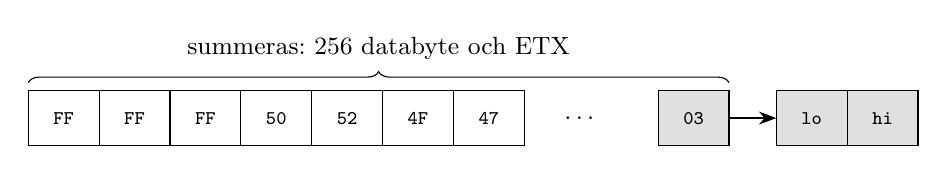
\begin{tikzpicture}[x=1mm,y=1mm]
\foreach \v/\x [count=\i] in {FF/0,FF/9,FF/18,50/27,52/36,4F/45,47/54} {
  \draw (\x,0) rectangle ++(9,7);
  \node[font=\scriptsize\ttfamily] at (\x+4.5,3.5) {\v};
}
\node[font=\small] at (70,3.5) {$\ldots$};
\draw[fill=gra] (80,0) rectangle ++(9,7) node[midway,font=\scriptsize\ttfamily] {03};
\draw[fill=gra] (95,0) rectangle ++(9,7) node[midway,font=\scriptsize\ttfamily] {lo};
\draw[fill=gra] (104,0) rectangle ++(9,7) node[midway,font=\scriptsize\ttfamily] {hi};
\draw[decorate,decoration={brace,amplitude=4pt}]
  (0,8) -- (89,8) node[midway,above=5pt,font=\small]
  {summeras: 256 databyte och ETX};
\draw[pil] (89,3.5) -- (95,3.5);
\end{tikzpicture}
\caption{Summan. Ett block med \kw{FF} och sedan 255 nollor ger
$255 + 3 = 258 =$ \adr{0102}, alltså \kw{02 01} på bandet.}
\end{figure}

Ett block från ABC80 är $256 + 8 \times 264 = 2\,368$ bitar och tar
ungefär 3,2~s.

\section{Filen}

En fil är ett filhuvud (namnblocket) och sedan datablock, numrerade från
0. Före filhuvudet låter ROM:en motorn gå i ungefär 6,8~s så att bandet
kommer upp i fart, och motorn går sedan hela tiden som filen är öppen.
Skriver programmet sällan blir det tystnad mellan blocken.

\begin{figure}[H]
\centering
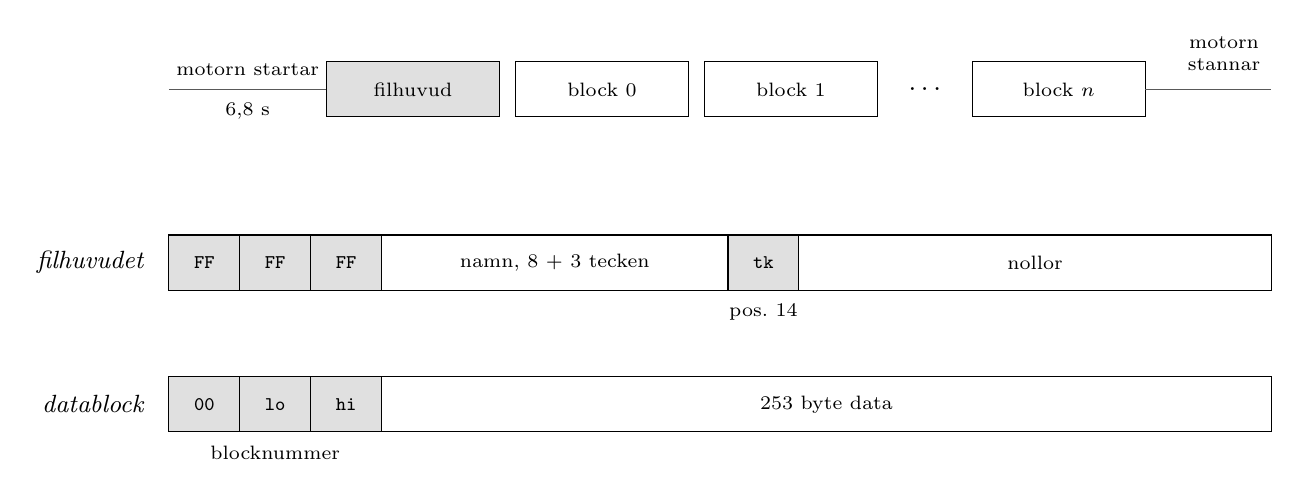
\begin{tikzpicture}[x=1mm,y=1mm]
\draw[mork] (0,3.5) -- (20,3.5);
\node[font=\scriptsize,above] at (10,4) {motorn startar};
\node[font=\scriptsize,below] at (10,3) {6,8 s};
\draw[fill=gra] (20,0) rectangle ++(22,7) node[midway,font=\scriptsize] {filhuvud};
\draw (44,0) rectangle ++(22,7) node[midway,font=\scriptsize] {block 0};
\draw (68,0) rectangle ++(22,7) node[midway,font=\scriptsize] {block 1};
\node at (96,3.5) {$\ldots$};
\draw (102,0) rectangle ++(22,7) node[midway,font=\scriptsize] {block $n$};
\draw[mork] (124,3.5) -- (140,3.5);
\node[font=\scriptsize,align=center] at (134,8) {motorn\\stannar};
% filhuvudet uppdelat
\begin{scope}[yshift=-22mm]
\foreach \v/\x/\w in {FF/0/9,FF/9/9,FF/18/9} \draw[fill=gra] (\x,0) rectangle ++(\w,7)
  node[midway,font=\scriptsize\ttfamily] {\v};
\draw (27,0) rectangle ++(44,7) node[midway,font=\scriptsize] {namn, 8 + 3 tecken};
\draw[fill=gra] (71,0) rectangle ++(9,7) node[midway,font=\scriptsize\ttfamily] {tk};
\draw (80,0) rectangle ++(60,7) node[midway,font=\scriptsize] {nollor};
\node[font=\scriptsize,anchor=north] at (75.5,-0.5) {pos.\ 14};
\end{scope}
\node[font=\small\itshape,anchor=east] at (-2,-18.5) {filhuvudet};
\begin{scope}[yshift=-40mm]
\draw[fill=gra] (0,0) rectangle ++(9,7) node[midway,font=\scriptsize\ttfamily] {00};
\draw[fill=gra] (9,0) rectangle ++(9,7) node[midway,font=\scriptsize\ttfamily] {lo};
\draw[fill=gra] (18,0) rectangle ++(9,7) node[midway,font=\scriptsize\ttfamily] {hi};
\draw (27,0) rectangle ++(113,7) node[midway,font=\scriptsize] {253 byte data};
\node[font=\scriptsize,anchor=north] at (13.5,-0.5) {blocknummer};
\end{scope}
\node[font=\small\itshape,anchor=east] at (-2,-36.5) {datablock};
\end{tikzpicture}
\caption{En fil på bandet, filhuvudet och ett datablock. Namnet fylls ut med
blanksteg. Position 14 är tidkonstanten för datablocken i ABC 800-serien;
ABC80 skriver en nolla där.}
\end{figure}

När ABC80 läser växlar ROM:en mellan två buffertar, \adr{FB00} och
\adr{FC00}. Läser programmet långsamt går bandet vidare medan båda är fulla,
och nästa block har då fel nummer (fel 37). Kommer inget block inom ungefär
8,5~s blir det fel 42.

\section{ABC 800-serien}

ABC 800 C/M, 802 och 806 skriver samma sorts FM, men med kretsar i stället
för program. SIO:ns kanal B går i teckensynkront läge med synken
\kw{16 02}, och FM-kodningen görs med vanliga TTL-kretsar på
processorkortet (schemat för ABC 800, blad 7). DTR i SIO:n drar
motorreläet.

\begin{figure}[H]
\centering
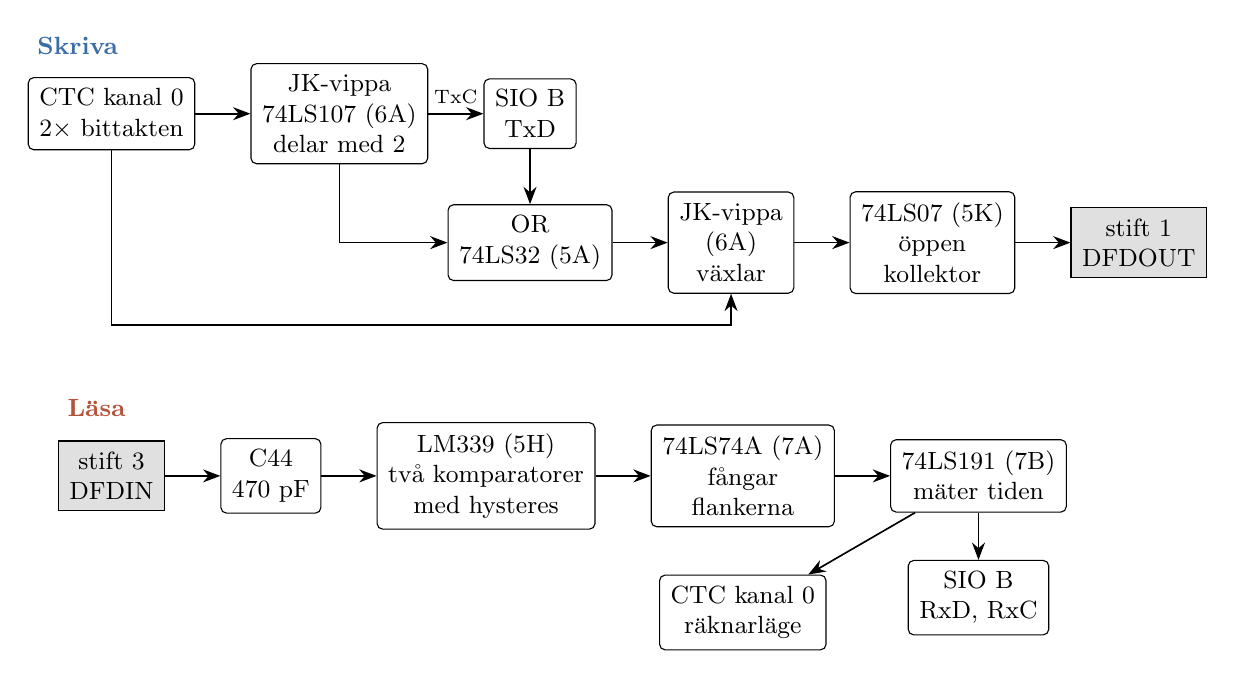
\begin{tikzpicture}[node distance=5mm and 7mm,every node/.style={font=\small}]
\node[ruta] (ctc) {CTC kanal 0\\$2\times$ bittakten};
\node[ruta,right=of ctc] (jk1) {JK-vippa\\74LS107 (6A)\\delar med 2};
\node[ruta,right=of jk1] (sio) {SIO B\\TxD};
\node[ruta,below=7mm of sio] (or) {OR\\74LS32 (5A)};
\node[ruta,right=of or] (jk2) {JK-vippa\\(6A)\\växlar};
\node[ruta,right=of jk2] (oc) {74LS07 (5K)\\öppen\\kollektor};
\node[fil,right=of oc] (out) {stift 1\\DFDOUT};
\draw[pil] (ctc) -- (jk1);
\draw[pil] (jk1) -- node[above,font=\scriptsize] {TxC} (sio);
\draw[pil] (jk1) |- (or);
\draw[pil] (sio) -- (or);
\draw[pil] (or) -- (jk2);
\draw[pil] (ctc.south) |- ($(jk2.south)+(0,-4mm)$) -- (jk2.south);
\draw[pil] (jk2) -- (oc);
\draw[pil] (oc) -- (out);
\begin{scope}[yshift=-46mm]
\node[fil] (in) {stift 3\\DFDIN};
\node[ruta,right=of in] (c44) {C44\\470 pF};
\node[ruta,right=of c44] (lm) {LM339 (5H)\\två komparatorer\\med hysteres};
\node[ruta,right=of lm] (ff) {74LS74A (7A)\\fångar\\flankerna};
\node[ruta,right=of ff] (cnt) {74LS191 (7B)\\mäter tiden};
\node[ruta,below=6mm of cnt] (sio2) {SIO B\\RxD, RxC};
\node[ruta,below=6mm of ff] (ctc2) {CTC kanal 0\\räknarläge};
\draw[pil] (in) -- (c44); \draw[pil] (c44) -- (lm); \draw[pil] (lm) -- (ff);
\draw[pil] (ff) -- (cnt); \draw[pil] (cnt) -- (sio2);
\draw[pil] (cnt) -- (ctc2);
\end{scope}
\node[anchor=west,font=\small\bfseries,text=fut] at ($(ctc.north west)+(0,4mm)$) {Skriva};
\node[anchor=west,font=\small\bfseries,text=fin] at ($(in.north west)+(0,4mm)$) {Läsa};
\end{tikzpicture}
\caption{FM i ABC 800-serien. Vid skrivning delar en vippa CTC:ns klocka
till bitklockan TxC. OR-grinden släpper igenom antingen den eller TxD till
nästa vippa, som växlar: alltid vid cellgränsen och mitt i cellen när
biten är 1. Vid läsning mäter en räknare tiden mellan flankerna och gör om
dem till RxD och RxC. Hur räknaren laddas går inte att läsa i skanningen
(?), och klockans väg till den andra vippan är förenklad.}
\end{figure}

Bitcellen blir $2 \times 16 \times \mathit{tk}$ T vid 3~MHz. Filhuvudet
skrivs och läses alltid med tk 129, ungefär 700 baud, och anger själv
tidkonstanten för datablocken på position 14. ABC 802 skriver 40, ungefär
2\,400 baud. Ett band från ABC80 har en nolla där, och då gör \namn{CASCTC}
ingenting: hela filen läses i 700 baud. Därför läser ABC 800 band från
ABC80.

\begin{center}
\small
\begin{tabular}{@{}lll@{}}
\toprule
Maskin & Var koden ligger & Källa \\
\midrule
ABC 802 & \namn{CAS:} på \adr{736D}--\adr{79C0} & den disassemblerade ROM:en \\
ABC 800 M & ROM 0: \namn{CASRD} \adr{0549}, \namn{CASWR} \adr{05DF}, \namn{CASCTC} \adr{0666} & jämförd med ABC 802 \\
ABC 800 C & ROM 0, omkring \adr{2F} lägre & \\
ABC 806 & ROM:en finns inte här (?) & manualerna \\
\bottomrule
\end{tabular}
\end{center}

\section{Innehållet}

Ett program sparat med \kw{SAVE} är BAC, kod som interpretatorn kör: med
första byten \adr{82} från ABC80 och \adr{8F} från BASIC II, som har ett
annat format. Med \kw{LIST} och \kw{PRINT~\#} blir det text, rader som
slutar med CR. LF skrivs inte, och två eller flera blanksteg i följd blir
\kw{09}~$n$. Texten står i datablockens 253 byte, högst 252 tecken och
sedan ETX.

\begin{figure}[H]
\centering
\begin{tikzpicture}[x=1mm,y=1mm]
\node[anchor=west,font=\small] at (0,12) {\kw{10 PRINT \textquotedbl A\ \ \ \ B\textquotedbl} och CR};
\foreach \v/\t [count=\i from 0] in {31/1,30/0,20/ ,50/P,52/R,49/I,4E/N,54/T,
  20/ ,22/\textquotedbl,41/A,09/,04/,42/B,22/\textquotedbl,0D/CR,03/ETX} {
  \draw (\i*8,0) rectangle ++(8,7) node[midway,font=\scriptsize\ttfamily] {\v};
  \node[font=\scriptsize\ttfamily,anchor=north] at (\i*8+4,-0.5) {\t};
}
\draw[fin,line width=0.8pt] (88,0) rectangle ++(16,7);
\end{tikzpicture}
\caption{En rad i ett textblock. De fyra blankstegen blir \kw{09 04}.
ETX avslutar texten i blocket, och vid läsning är \kw{00} slut på filen.}
\end{figure}

Bokstäverna ÄÖÅÜÉ är den svenska 7-bitarskoden: \kw{[\textbackslash]}
blir ÄÖÅ, \kw{\{|\}} äöå, \kw{@} É, \kw{`} é, \kw{\textasciicircum} Ü och
\kw{\textasciitilde} ü. I dag skrivs filerna oftast i UTF-8 med LF, och i
MS-DOS i teckentabell 850 med CR LF.

\section{Verktygen}

Verktygen finns i Python 3 (\kw{python/}) och i C89 (\kw{c/}), med samma
namn, flaggor och utdata. Mellanformatet är \kw{.kas}: blockens 256 byte
efter varandra, utan inramning.

\begin{figure}[H]
\centering
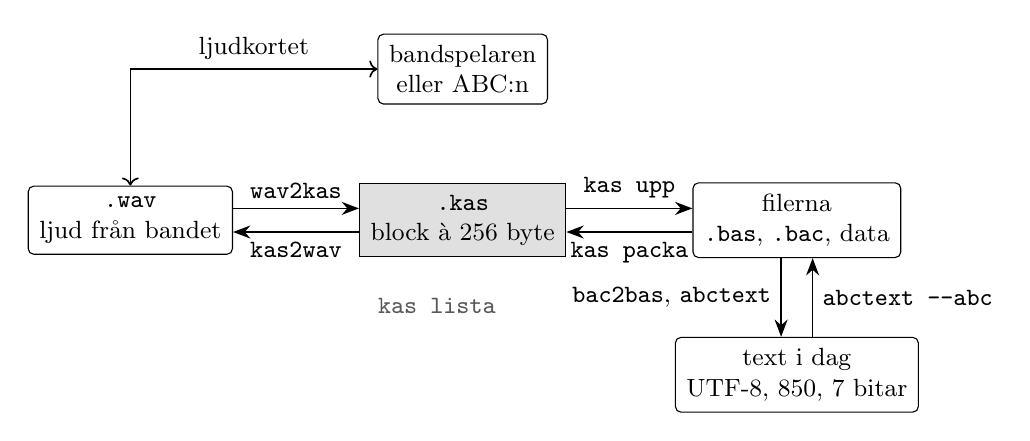
\begin{tikzpicture}[node distance=6mm and 16mm,every node/.style={font=\small}]
\node[fil,minimum width=22mm,minimum height=9mm] (kas) {\kw{.kas}\\block à 256 byte};
\node[ruta,left=of kas,minimum width=22mm] (wav) {\kw{.wav}\\ljud från bandet};
\node[ruta,right=of kas,minimum width=24mm] (filer) {filerna\\\kw{.bas}, \kw{.bac}, data};
\node[ruta,below=10mm of filer] (txt) {text i dag\\UTF-8, 850, 7 bitar};
\node[ruta,above=10mm of kas] (bandsp) {bandspelaren\\eller ABC:n};
\draw[pil] ([yshift=1.5mm]wav.east) -- node[above] {\kw{wav2kas}} ([yshift=1.5mm]kas.west);
\draw[pil] ([yshift=-1.5mm]kas.west) -- node[below] {\kw{kas2wav}} ([yshift=-1.5mm]wav.east);
\draw[pil] ([yshift=1.5mm]kas.east) -- node[above] {\kw{kas upp}} ([yshift=1.5mm]filer.west);
\draw[pil] ([yshift=-1.5mm]filer.west) -- node[below] {\kw{kas packa}} ([yshift=-1.5mm]kas.east);
\draw[pil] ([xshift=-2mm]filer.south) -- node[left] {\kw{bac2bas}, \kw{abctext}} ([xshift=-2mm]txt.north);
\draw[pil] ([xshift=2mm]txt.north) -- node[right] {\kw{abctext --abc}} ([xshift=2mm]filer.south);
\draw[pil,<->] (bandsp) -| node[pos=0.25,above] {ljudkortet} (wav);
\node[font=\small,anchor=north west,text=mork] at ($(kas.south)+(-12mm,-4mm)$) {\kw{kas lista}};
\end{tikzpicture}
\caption{Verktygen och formaten. \kw{wav2kas} läser både ABC80 och
ABC 800-serien och väljer själv tidkonstanten ur filhuvudet.
\kw{kas2wav --abc800} skriver i ABC 800-seriens takt, och \kw{--tk} väljer
tidkonstanten för datablocken.}
\end{figure}

Några exempel:

\begin{center}
\small
\begin{tabular}{@{}>{\ttfamily}l l@{}}
\toprule
\normalfont Kommando & Gör \\
\midrule
wav2kas -o band.kas band.wav & ljudet blir block \\
kas lista band.kas & filerna och blocken \\
kas upp -d ut band.kas & varje fil för sig \\
bac2bas ut/PROG.BAC & BAC blir text, som \kw{LIST} \\
abctext ut/PROG.BAS & 7 bitar och CR blir UTF-8 och LF \\
kas packa -o ny.kas PROG.BAS & en fil blir block, som ROM:en packar \\
kas2wav --abc800 --tk 40 ny.kas & block blir ljud för ABC 802 i 2\,400 baud \\
\bottomrule
\end{tabular}
\end{center}

\section{Hårdvaran}

Två förslag, inte byggda (se \kw{HARDVARA.md}). Det första är en kabel
till ljudkortet: en delare ned till linjenivå från DFDOUT, och ett motstånd
in till DFDIN, där C44 i datorn tar bort likspänningen. ABC80 behöver
troligen en komparator på ingången (?). Det andra är en Raspberry Pi Pico
med ett SD-kort som tar bandspelarens plats och använder samma kod som
verktygen.

\begin{figure}[H]
\centering
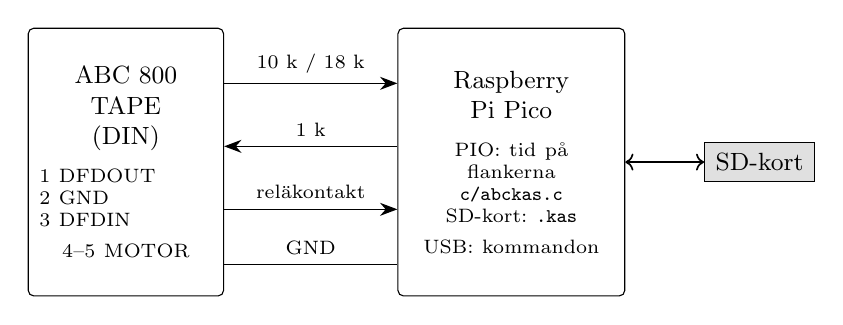
\begin{tikzpicture}[node distance=6mm and 12mm,every node/.style={font=\small}]
\node[ruta,minimum height=34mm,text width=22mm] (abc) {ABC 800\\TAPE\\(DIN)\\[2mm]
  \raggedright\scriptsize 1 DFDOUT\\2 GND\\3 DFDIN\\4--5 MOTOR};
\node[ruta,right=22mm of abc,minimum height=34mm,text width=26mm] (pico)
  {Raspberry Pi Pico\\[2mm]\scriptsize PIO: tid på flankerna\\
   \kw{c/abckas.c}\\SD-kort: \kw{.kas}\\USB: kommandon};
\node[fil,right=10mm of pico] (sd) {SD-kort};
\draw[pil] ($(abc.east)+(0,10mm)$) -- node[above,font=\scriptsize] {10 k / 18 k} ($(pico.west)+(0,10mm)$);
\draw[pil] ($(pico.west)+(0,2mm)$) -- node[above,font=\scriptsize] {1 k} ($(abc.east)+(0,2mm)$);
\draw[pil] ($(abc.east)+(0,-6mm)$) -- node[above,font=\scriptsize] {reläkontakt} ($(pico.west)+(0,-6mm)$);
\draw ($(abc.east)+(0,-13mm)$) -- node[above,font=\scriptsize] {GND} ($(pico.west)+(0,-13mm)$);
\draw[pil,<->] (pico) -- (sd);
\end{tikzpicture}
\caption{Picon som bandspelare. Delaren tar DFDOUT från 5 V ned till 3,2 V.
Motorkontakten drar en ingång till jord när datorn vill ha bandet: kommer
det signal spelar Picon in, annars spelar den upp nästa fil.}
\end{figure}

\section*{Källor}

\small
ROM:erna för ABC80 (\kw{abc80old.asm}: \namn{CASPRE}, \namn{CASWBL},
\namn{CASWBI}, \namn{CASRBL}, \namn{RCVSTA}, \namn{CASINT}, \namn{RCVBLK}),
ABC 802 (\namn{CASRD}, \namn{CASWR}, \namn{CASCTC}) och ABC 800 M och C
(ROM 0). Luxor, schemat för ABC 800, blad 7, ``Processor unit'' 55\,10788.
Luxor, \emph{ABC 800 bruksanvisning}, avsnitten om ABC 820. Luxor,
servicemanualen för ABC80. Gunnar Markesjö, \emph{Mikrodatorns ABC}, 1978,
s.~112--124, 164--167 och 193--194. Provet mot de elva riktiga banden och
emulatorerna står i \kw{README.md}.

\end{document}
